\documentclass{article}

\usepackage{authblk} % for multiple authors and affiliations
\usepackage{graphicx} % to inlcude graphics with \includegraphics
\usepackage{tikz}
\usepackage{listings}
%\usepackage{geometry}
\usepackage[utf8]{inputenc}
\usepackage[T1]{fontenc}
\usepackage{fourier}


%New colors defined below
\definecolor{codegreen}{rgb}{0,0.6,0}
\definecolor{codegray}{rgb}{0.5,0.5,0.5}
\definecolor{codepurple}{rgb}{0.58,0,0.82}
\definecolor{backcolour}{rgb}{0.95,0.95,0.92}

%Code listing style named "mystyle"
\lstdefinestyle{mystyle}{
  backgroundcolor=\color{backcolour}, commentstyle=\color{codegreen},
  keywordstyle=\color{magenta},
  numberstyle=\tiny\color{codegray},
  stringstyle=\color{codepurple},
  basicstyle=\ttfamily\footnotesize,
  breakatwhitespace=false,         
  breaklines=true,                 
  captionpos=b,                    
  keepspaces=true,                 
  numbers=left,                    
  numbersep=5pt,                  
  showspaces=false,                
  showstringspaces=false,
  showtabs=false,                  
  tabsize=2
}

%"mystyle" code listing set
\lstset{style=mystyle}

\author{\textbf{MD ARIF HOSSAIN}}









\title{\textbf {Rubik's Cube - An Application of Group Theory}}
%\affil{Department of Mathematics, Shahjalal University of Science and Technology, Sylhet, Bangladesh.}

\date{}



\begin{document}

\maketitle

   \section*{Abstract} 
 Erno Rubik is the inventor of the popular puzzle known as the Rubik's Cube. One of the most well-liked gadgets ever is this one. Additionally, the Rubik's cube's math is impressive.Group Theory is the basis for each and every solved cube. How they are aligned and permuted can be determined by the group theory. This paper explores the mathematics underlying the Rubik's cube solve as well as how the cube functions as a group.
 \section{Introduction}
From 1971 to 1979, Rubik was a professor of architecture at the Budapest College of Applied Arts (Iparművészeti Főiskola). It was during his time there that he built designs for a three-dimensional puzzle and completed the first working prototype of the Rubik's Cube in 1974, applying for a patent on the puzzle in 1975.Today Rubik's Cube is more popular and speed cubing competitions are held through the World Cube Association where different types of cube to solve and participant attempt to solve the cube as fast as possible. There are many types of cube like as "2*2*2 cube" , "3*3*3 (Rubik's Cube)" And other types of wca (world cube association) and other twisty puzzles.\cite{demaine2011algorithms}The cube has been studied in various field such as computer science and mathematics.In mathematics,the rubik's cube can be described as group theory. The different transformations and configurations of the cube from a subgroup of a permutation group generated by the different horizontal and vertical rotation of the puzzle.\cite{demaine2011algorithms}
The solution to the cube can also be described by Group
Theory.\cite{joyner2008adventures}
Group Theory allows for the examination of how the cube functions and
how the twists and turns return the cube to its solved state.

\section{Group}
To properly understand the Rubik's cube, we must first understand group theory.
\subsection{Group}
\subsubsection{Definition}
Let $G$ be a set together with a binary operation (usually called multiplication) that assigns to each ordered pair $(a, b)$ of elements of $G$ an element in $G$ denoted by $ab$.\\ We say G is a group under this operation if the following four properties are satisfied.\\
1.Closure: If $a$ and $b$ are two components in the group, $G$, then the product “$a * b$” is also in “$G$”.\\
2. Associativity: The operation is associative; that is, $(ab)c = a(bc)$ for
all $a, b, c$ in $G$.\\
3. Identity: There is an element e (called the identity) in $G$ such that
$ae = ea = a$ for all $a$ in $G$.\\
4. Inverses: For each element a in $G$, there is an element $b$ in $G$ (called
an inverse of $a$) such that $ab = ba = e$.\cite{gallian2021contemporary}
\section{How Rubik's Cube is related to the group structure ?}
\subsection{Introduction to Rubik's Cube}
A standard Rubik's Cube measures 5.6 centimetres (2+1⁄4 in) on each side.\cite{ins} The puzzle consists of 26 unique miniature cubes, also known as "cubies" or "cubelets". Each of these includes a concealed inward extension that interlocks with the other cubes while permitting them to move to different locations. However, the centre cube of each of the six faces is merely a single square façade; all six are affixed to the core mechanism. These provide structure for the other pieces to fit into and rotate around. Hence, there are 21 pieces: a single core piece consisting of three intersecting axes holding the six centre squares in place but letting them rotate, and 20 smaller plastic pieces that fit into it to form the assembled puzzle.\cite{zeng2018overview}
\begin{figure}[h!]
    \centering
    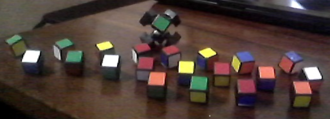
\includegraphics[width=4cm]{Disassembled_Rubik's_Cube_on_table,_16_June_2013.png}
    \caption{Disassembled Rubik's Cube}
    \label{fig:Rubiks Cube}
\end{figure}



There are six central pieces that show one coloured face, twelve edge pieces that show two coloured faces, and eight corner pieces that show three coloured faces. Each piece shows a unique colour combination, but not all combinations are present (for example, if red and orange are on opposite sides of the solved Cube, there is no edge piece with both red and orange sides). The location of these cubes relative to one another can be altered by twisting an outer third of the Cube by increments of 90 degrees, but the location of the coloured sides relative to one another in the completed state of the puzzle cannot be altered; it is fixed by the relative positions of the centre squares. However, Cubes with alternative colour arrangements also exist; for example, with the yellow face opposite the green, the blue face opposite the white, and red and orange remaining opposite each other.
\begin{figure}[h!]
    \centering
    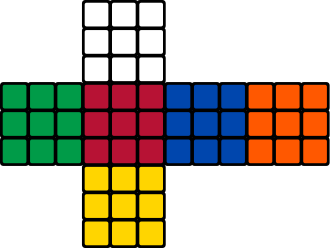
\includegraphics[width=4cm]{330px-Rubik's_cube_colors.svg.png}
    \caption{All the six color of a rubiks cube}
    \label{fig:Rubiks Cube}
\end{figure}
\begin{figure}[h!]
    \centering
    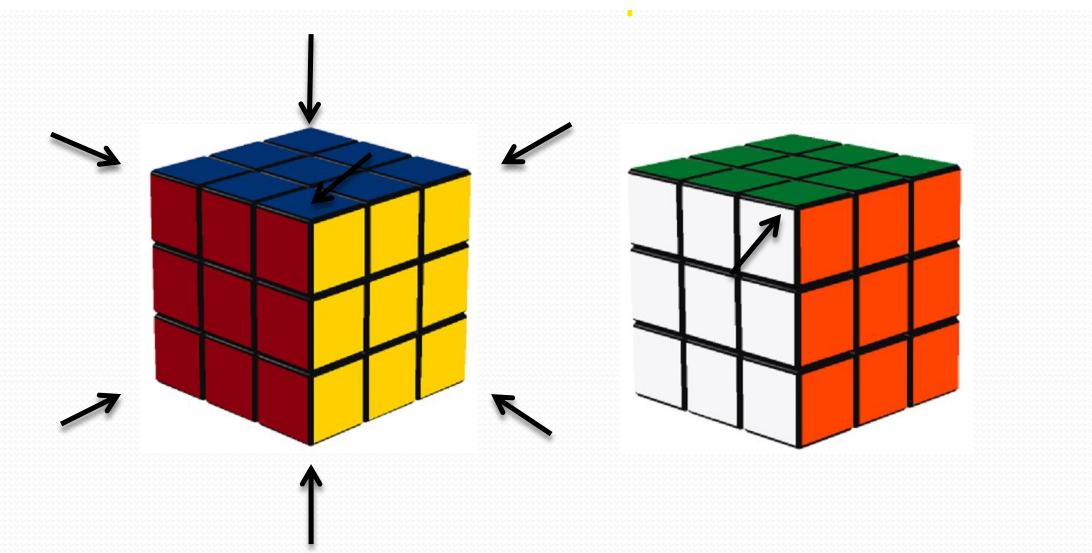
\includegraphics[width=4cm]{Screenshot 2023-07-05 230818.png}
    \caption{All the corners of a cube}
    \label{fig:Rubiks Cube}
\end{figure}
\begin{figure}[h!]
    \centering
    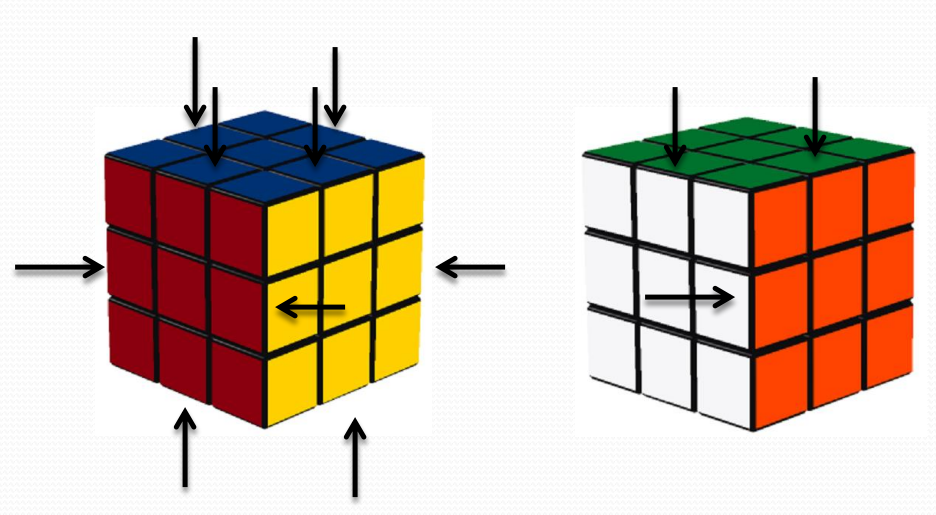
\includegraphics[width=4cm]{Screenshot 2023-07-05 230948.png}
    \caption{All the edge of a cube}
    \label{fig:Rubiks Cube}
\end{figure}\\
\subsection{Singmaster Notation}
Many 3×3×3 Rubik's Cube enthusiasts use a notation developed by \textbf{David Singmaster} to denote a sequence of moves, referred to as "Singmaster notation".\cite{flath2003adventures} Its relative nature allows algorithms to be written in such a way that they can be applied regardless of which side is designated the top or how the colours are organised on a particular cube.
\begin{itemize}
    \item F (Front): the side currently facing the solver
    \item B (Back): the side opposite the front
    \item U (Up): the side above or on top of the front side
    \item D (Down): the side opposite the top, underneath the Cube
    \item L (Left): the side directly to the left of the front
    \item R (Right): the side directly to the right of the front
    \item f (Front two layers): the side facing the solver and the corresponding middle layer
    \item b (Back two layers): the side opposite the front and the corresponding middle layer
    \item u (Up two layers): the top side and the corresponding middle layer
    \item d (Down two layers): the bottom layer and the corresponding middle layer
    \item l (Left two layers): the side to the left of the front and the corresponding middle layer
    \item r (Right two layers): the side to the right of the front and the corresponding middle layer
    \item x (rotate): rotate the entire Cube on R
    \item y (rotate): rotate the entire Cube on U
    \item z (rotate): rotate the entire Cube on F
\end{itemize}\\
When a prime symbol \textbf{" ' "} follows a letter, it denotes an anticlockwise face turn; while a letter without a prime symbol denotes a clockwise turn. These directions are as one is looking at the specified face. A letter followed by a $2$ (occasionally a superscript $2$) denotes two turns, or a 180-degree turn. R is right side clockwise, but R′ is right side anticlockwise. The letters $x$, $y$, and $z$ are used to indicate that the entire Cube should be turned about one of its axes, corresponding to R, U, and F turns respectively. When $x$, $y$, or $z$ is primed, it is an indication that the cube must be rotated in the opposite direction. When $x$, $y$, or $z$ is squared, the cube must be rotated $180$ degrees.\\
\begin{figure}[h!]
    \centering
    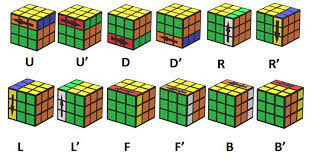
\includegraphics[width=4cm]{cube notation.jpg}
    \caption{Notation of Rubik's Cube}
    \label{fig:Rubiks Cube}
\end{figure}

The most common deviation from Singmaster notation, and in fact the current official standard, is to use "w", for "wide", instead of lowercase letters to represent moves of two layers; thus, a move of Rw is equivalent to one of r.\cite{cuberubik}

For methods using middle-layer turns (particularly corners-first methods), there is a generally accepted "MES" extension to the notation where letters M, E, and S denote middle layer turns. It was used e.g. in Marc Waterman's Algorithm.\cite{cuberubik2}

\begin{itemize}
    \item M (Middle): the layer between L and R, turn direction as L (top-down)
    \item E (Equator): the layer between U and D, turn direction as D (left-right)
    \item S (Standing): the layer between F and B, turn direction as F
\end{itemize}
\begin{center}
    \begin{figure}[htp]
    \centering
    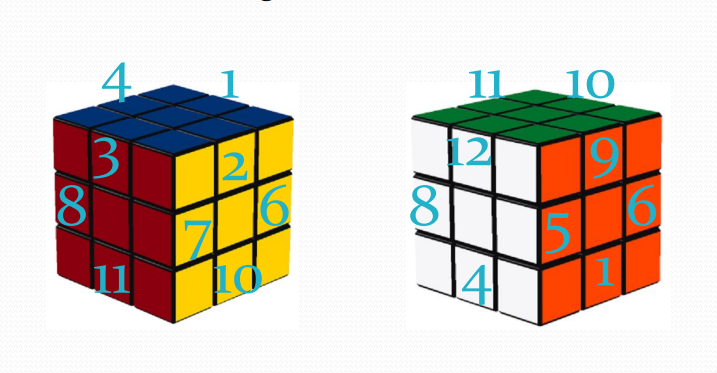
\includegraphics[width=4cm]{numbering corners.png}
    \caption{Numbering The Edge pieces}
    \label{fig:Rubiks Cube}
\end{figure}
\begin{figure}[htp]
    \centering
    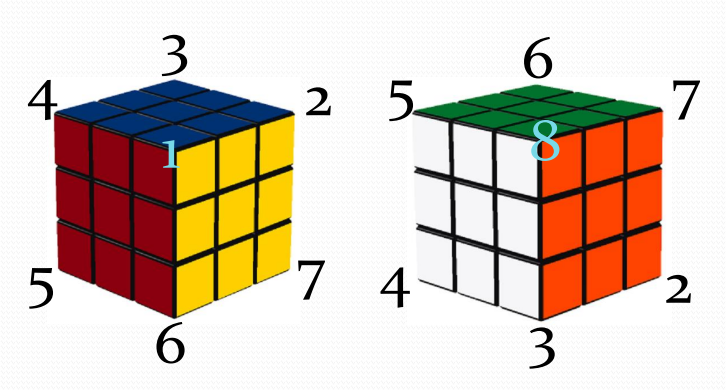
\includegraphics[width=4cm]{numbering edges.png}
    \caption{Numbering the corner pieces}
    \label{fig:Rubiks Cube}
\end{figure}
\end{center}
\subsection{Group Theory Part}
\textbf{1.Closure:} If $a$ and $b$ are two components in the group, $G$, then the product “$a * b$” is also in “$G$”.\\
Let's Suppose two move form the group structure or the rubik's cube move $< R , L , U , D , F , B  >$,if we took any two sequence or any two individual move if we perform them we will find the complete sequence in the closed group $ a * b $ which belongs to G\\
\begin{figure}[h!]
    \centering
    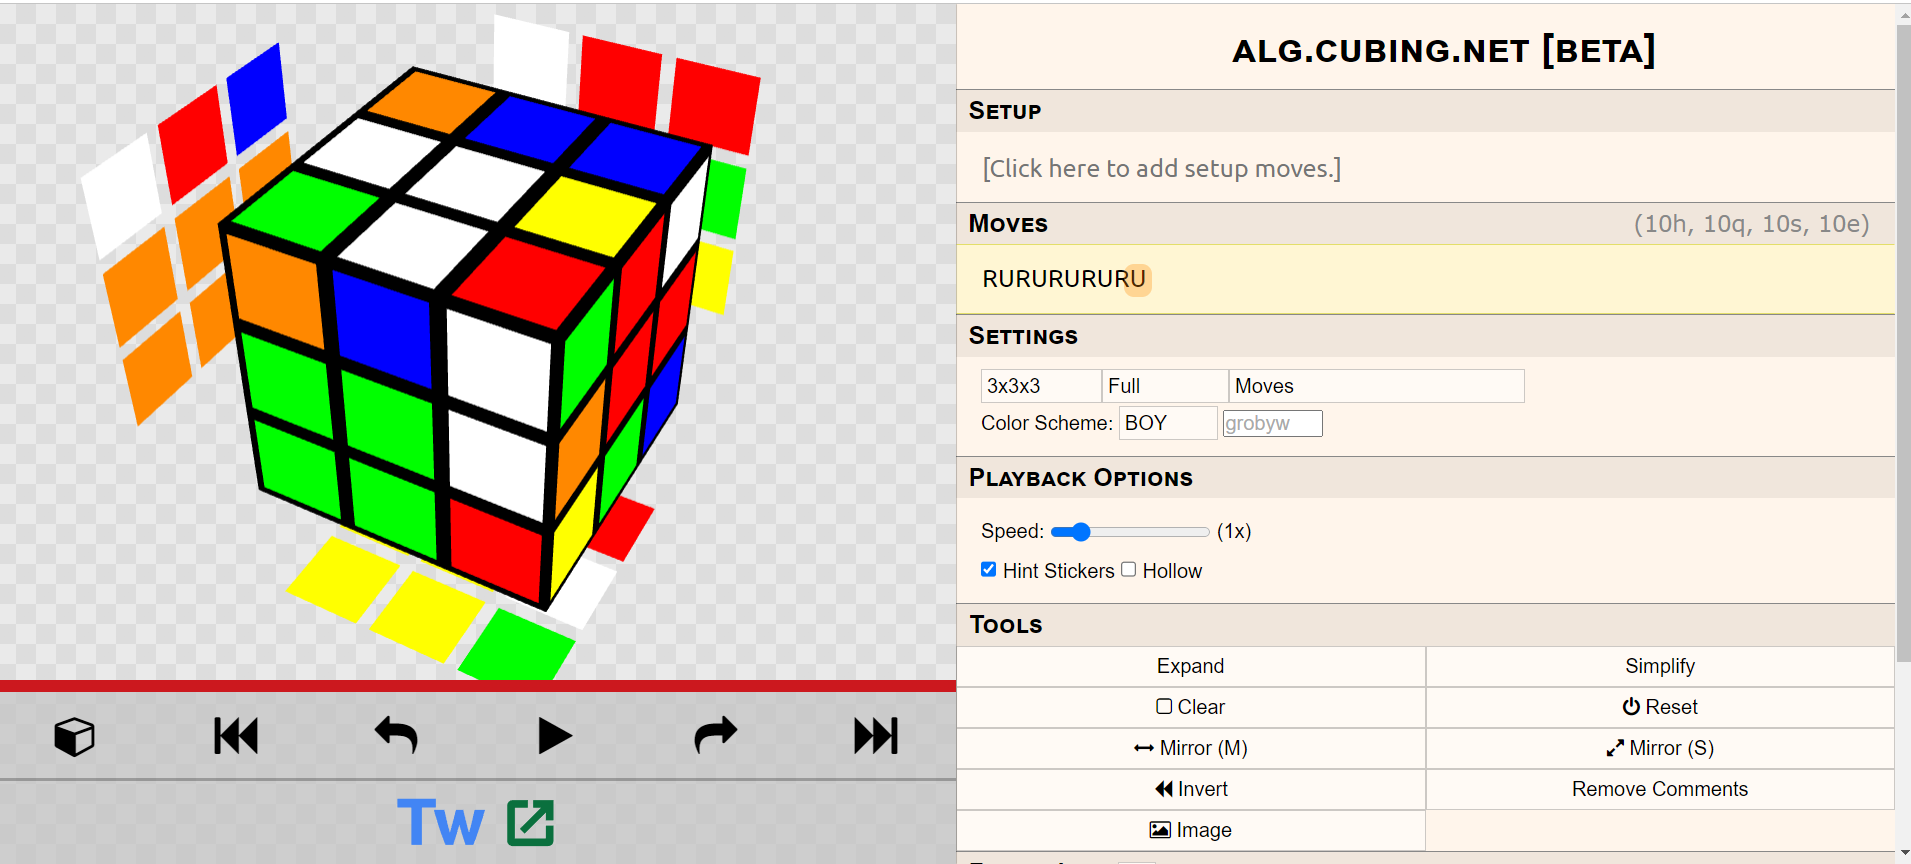
\includegraphics[width = 10cm ]{Screenshot 2023-07-06 000454.png}
    \caption{Performing any sequence}
    \label{fig:Rubiks Cube}
\end{figure}
$a = RURUR $ and $b = URURU$\\
$a * b = RURUR URURU $\\
\textbf{2. Associativity:} If $a$ and $b$ are two components in the group, $G$, then the product “$a * b$” is also in “$G$”.\\ The operation is associative; that is, $(a * b)c = a(b * c)$ for
all $a, b, c$ in $G$.\\
$ a = RU $
$ b = R'U' $
$c = R U$\\
\begin{center}
    \begin{figure}[h!]
    \centering
    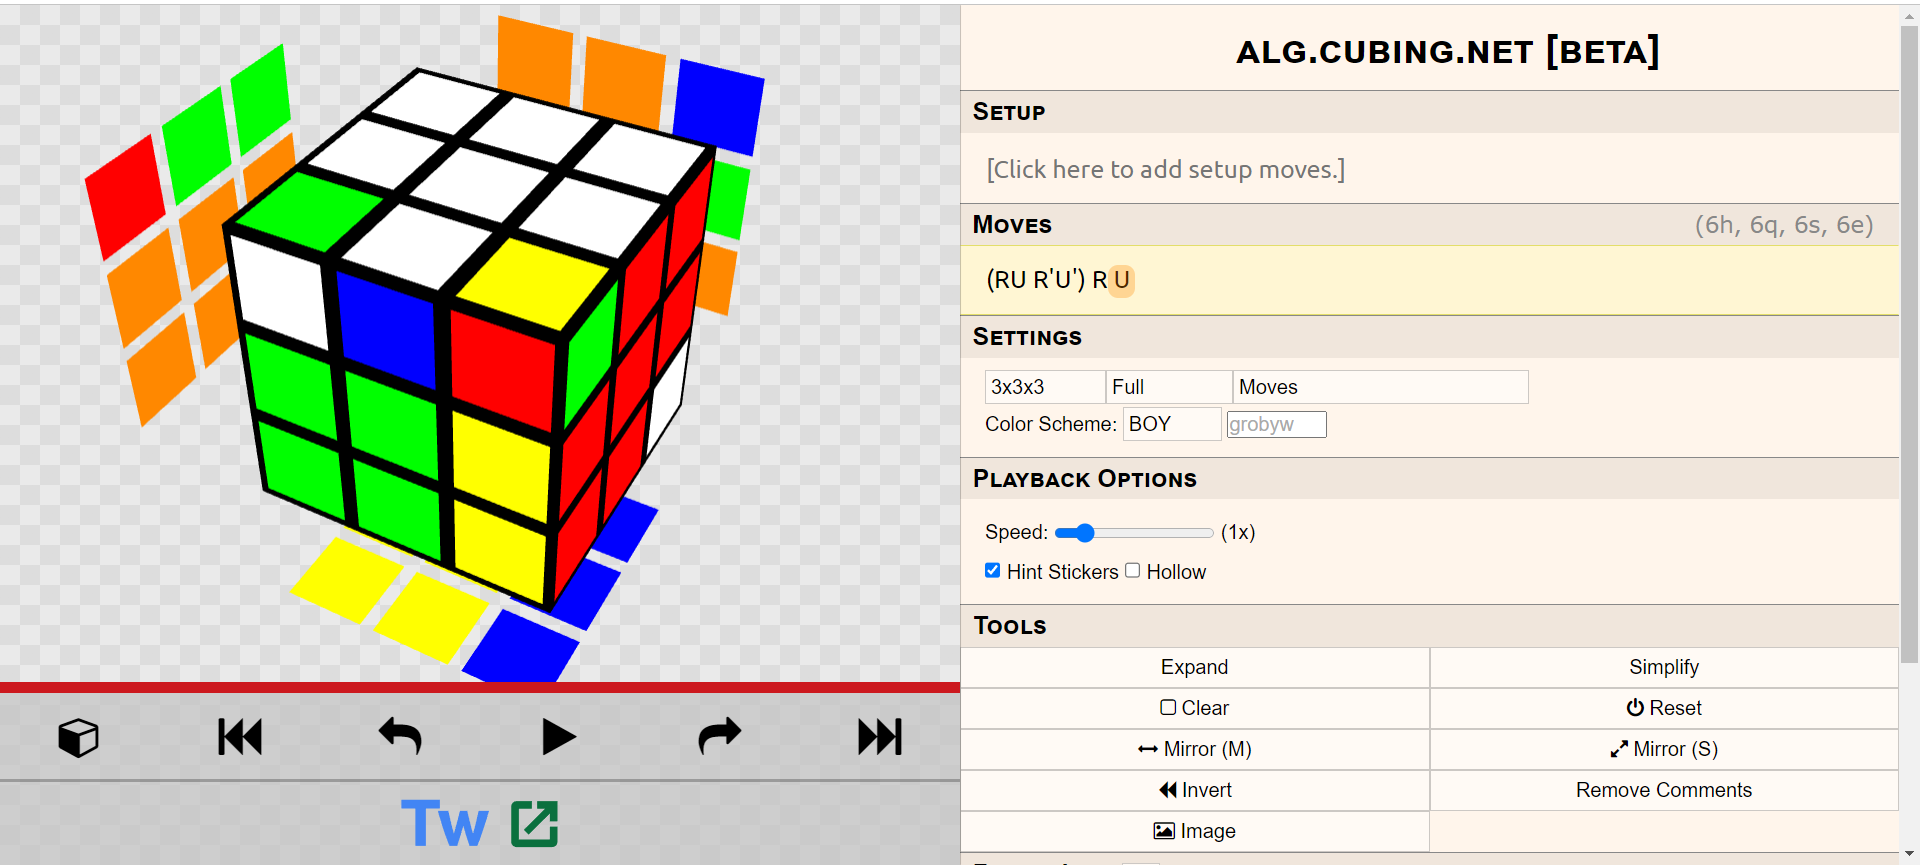
\includegraphics[width = 10cm ]{Screenshot 2023-07-06 001036.png}
    \caption{(RU R'U') R U or $ (a * b)*c $}
    \label{(RU R'U') R U or $ (a * b)*c $}
\end{figure}
\begin{figure}[h!]
    \centering
    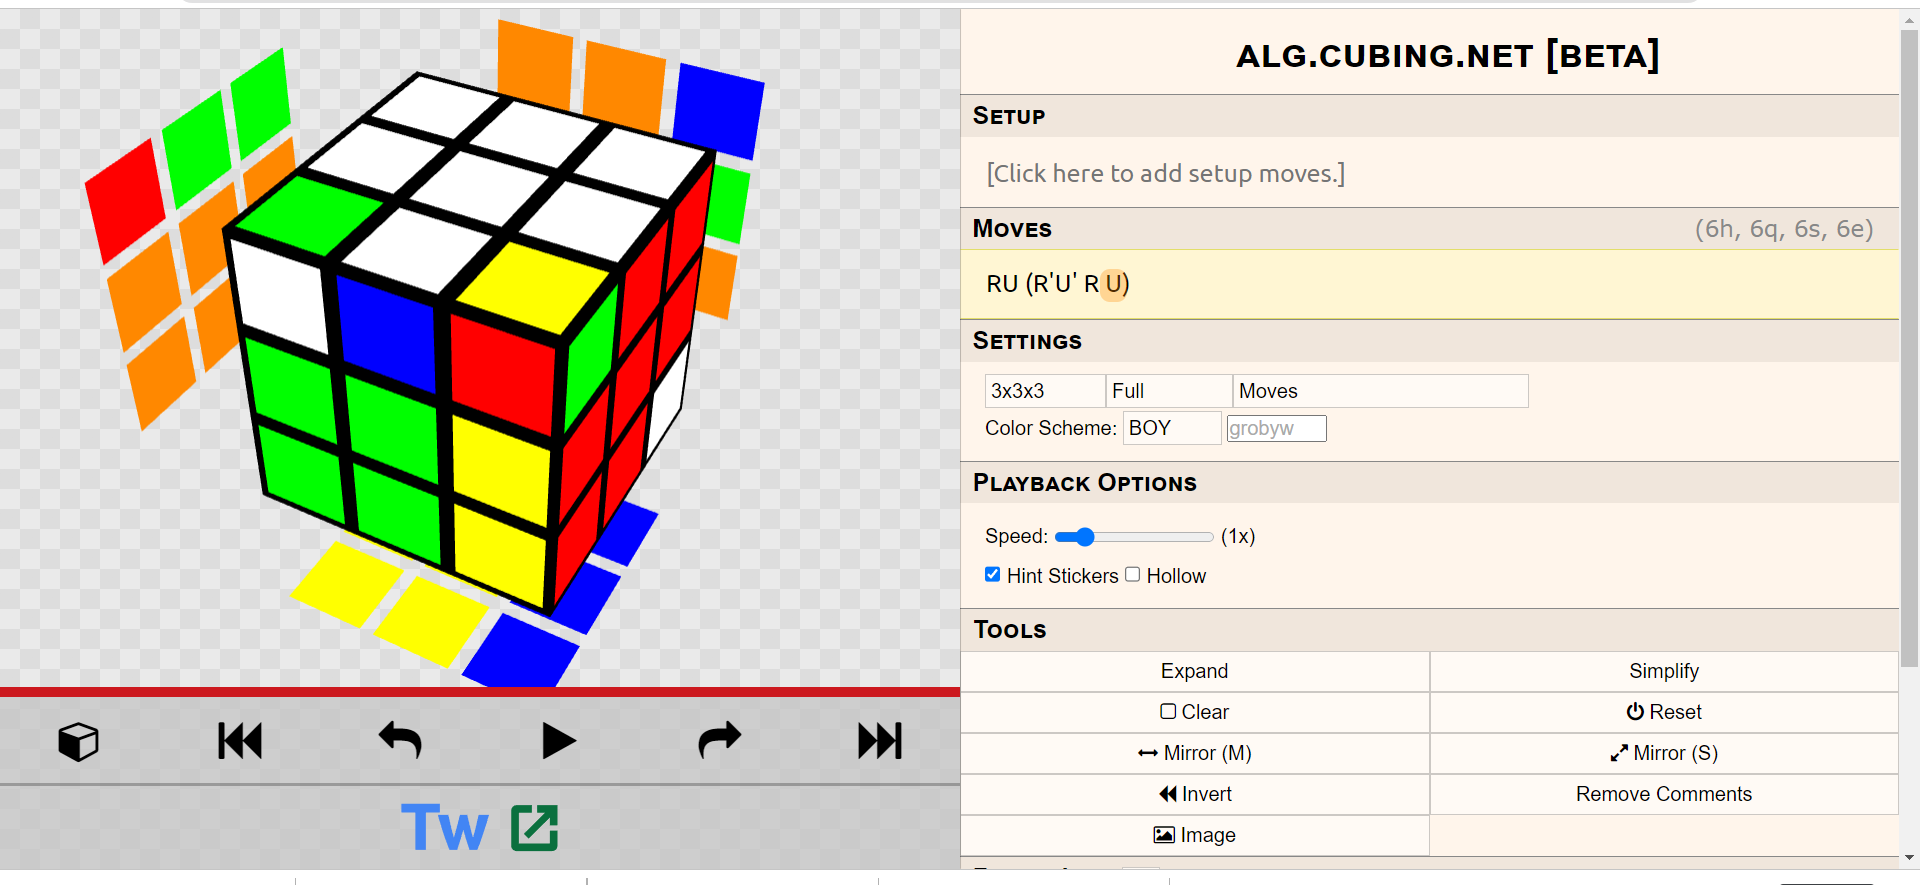
\includegraphics[width = 10cm ]{Screenshot 2023-07-06 001958.png}
    \caption{R U (R'U' R U) or $ a * (b *c) $}
    \label{(RU R'U') R U or $ (a * b)*c $}
\end{figure}
\end{center}
We can clearly see that it also holds the Associativity property\\\\\\\\\\
\textbf{3. Identity:} There is an element e (called the identity) in $G$ such that
$ae = ea = a$ for all $a$ in $G$.\\
\begin{figure}[h!]
    \centering
    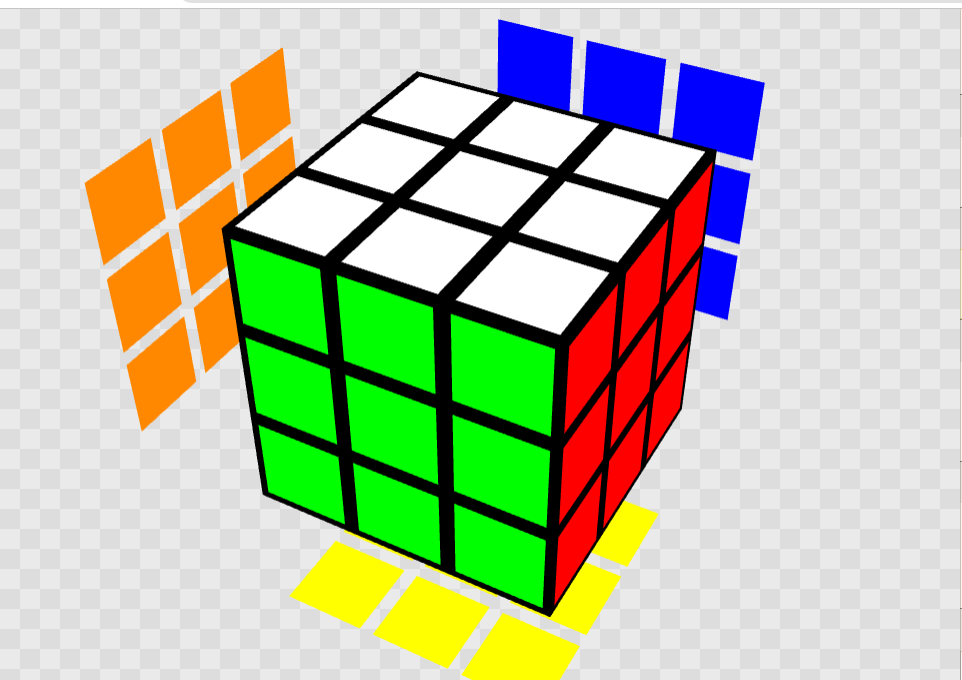
\includegraphics[width = 10cm ]{Screenshot 2023-07-06 003851.png}
    \caption{The Identity Element}
    \label{(RU R'U') R U or $ (a * b)*c $}
\end{figure}


\textbf{4. Inverses:}For each element a in $G$, there is an element $b$ in $G$ (called
an inverse of $a$) such that $ab = ba = e$.\\
\begin{figure}[h!]
    \centering
    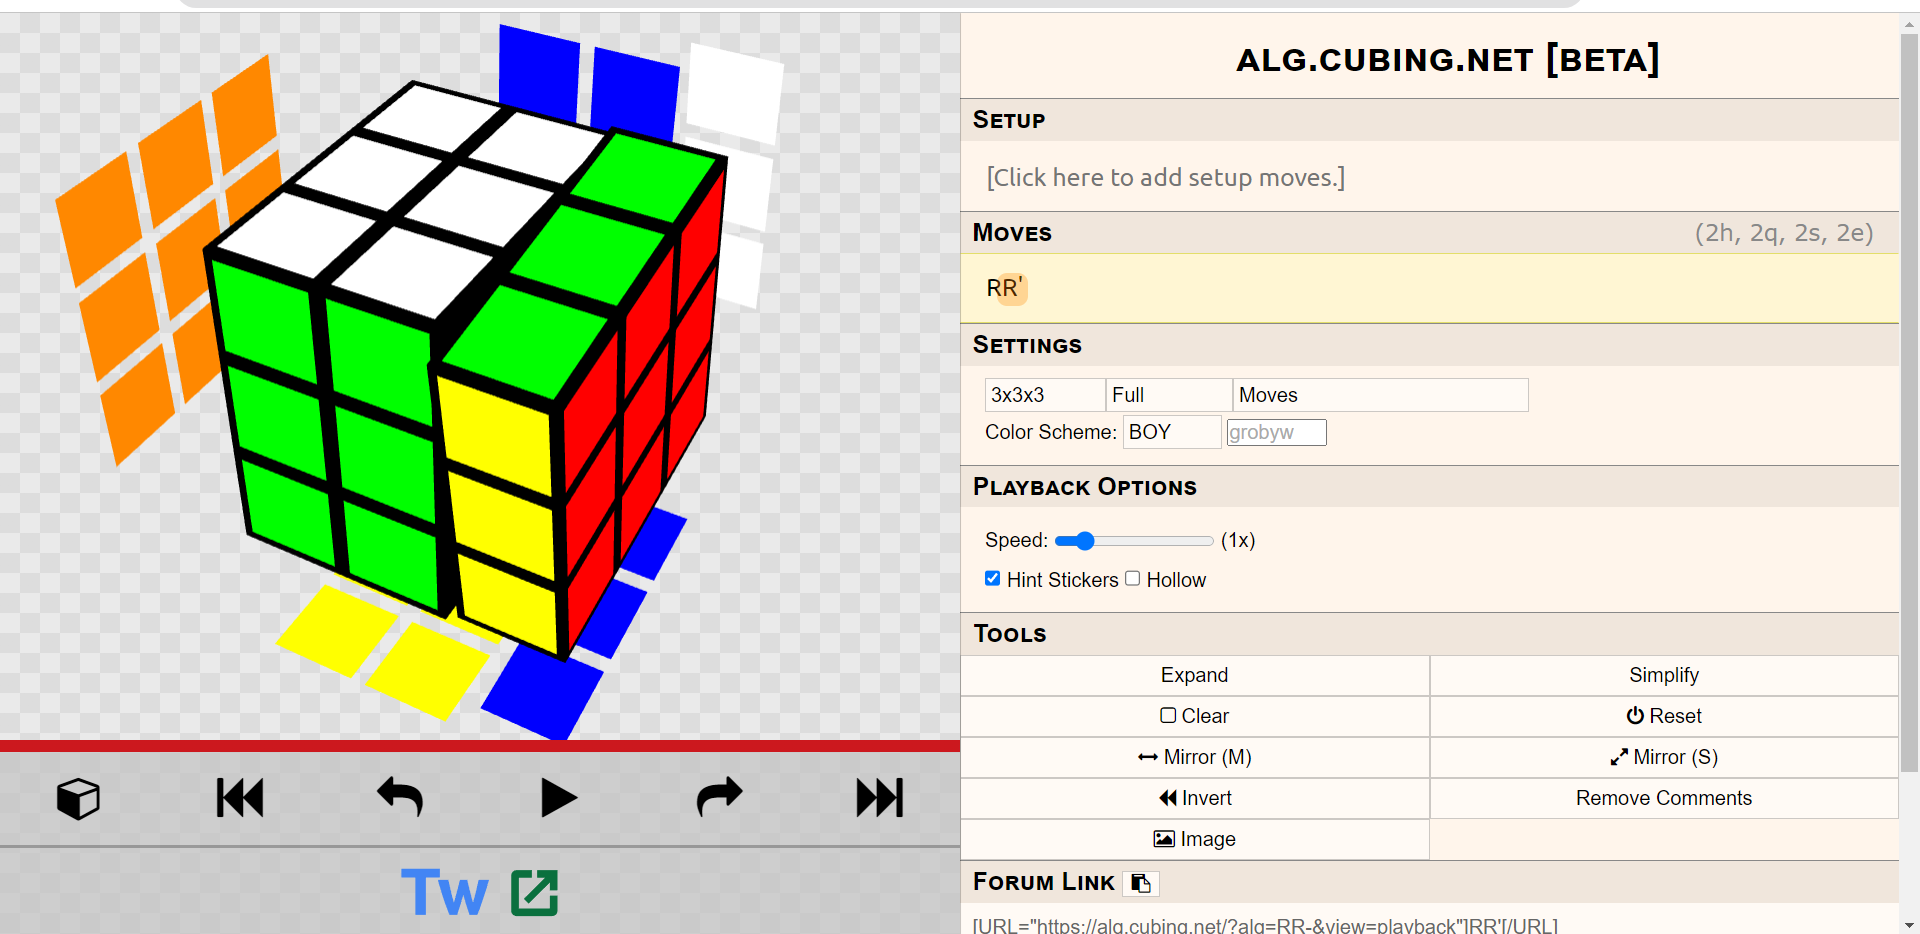
\includegraphics[width = 10cm ]{Screenshot 2023-08-16 153653.png}
    \caption{Performing a random move like R}
    \label{(RU R'U') R U or $ (a * b)*c $}
\end{figure}
\begin{figure}[h!]
    \centering
    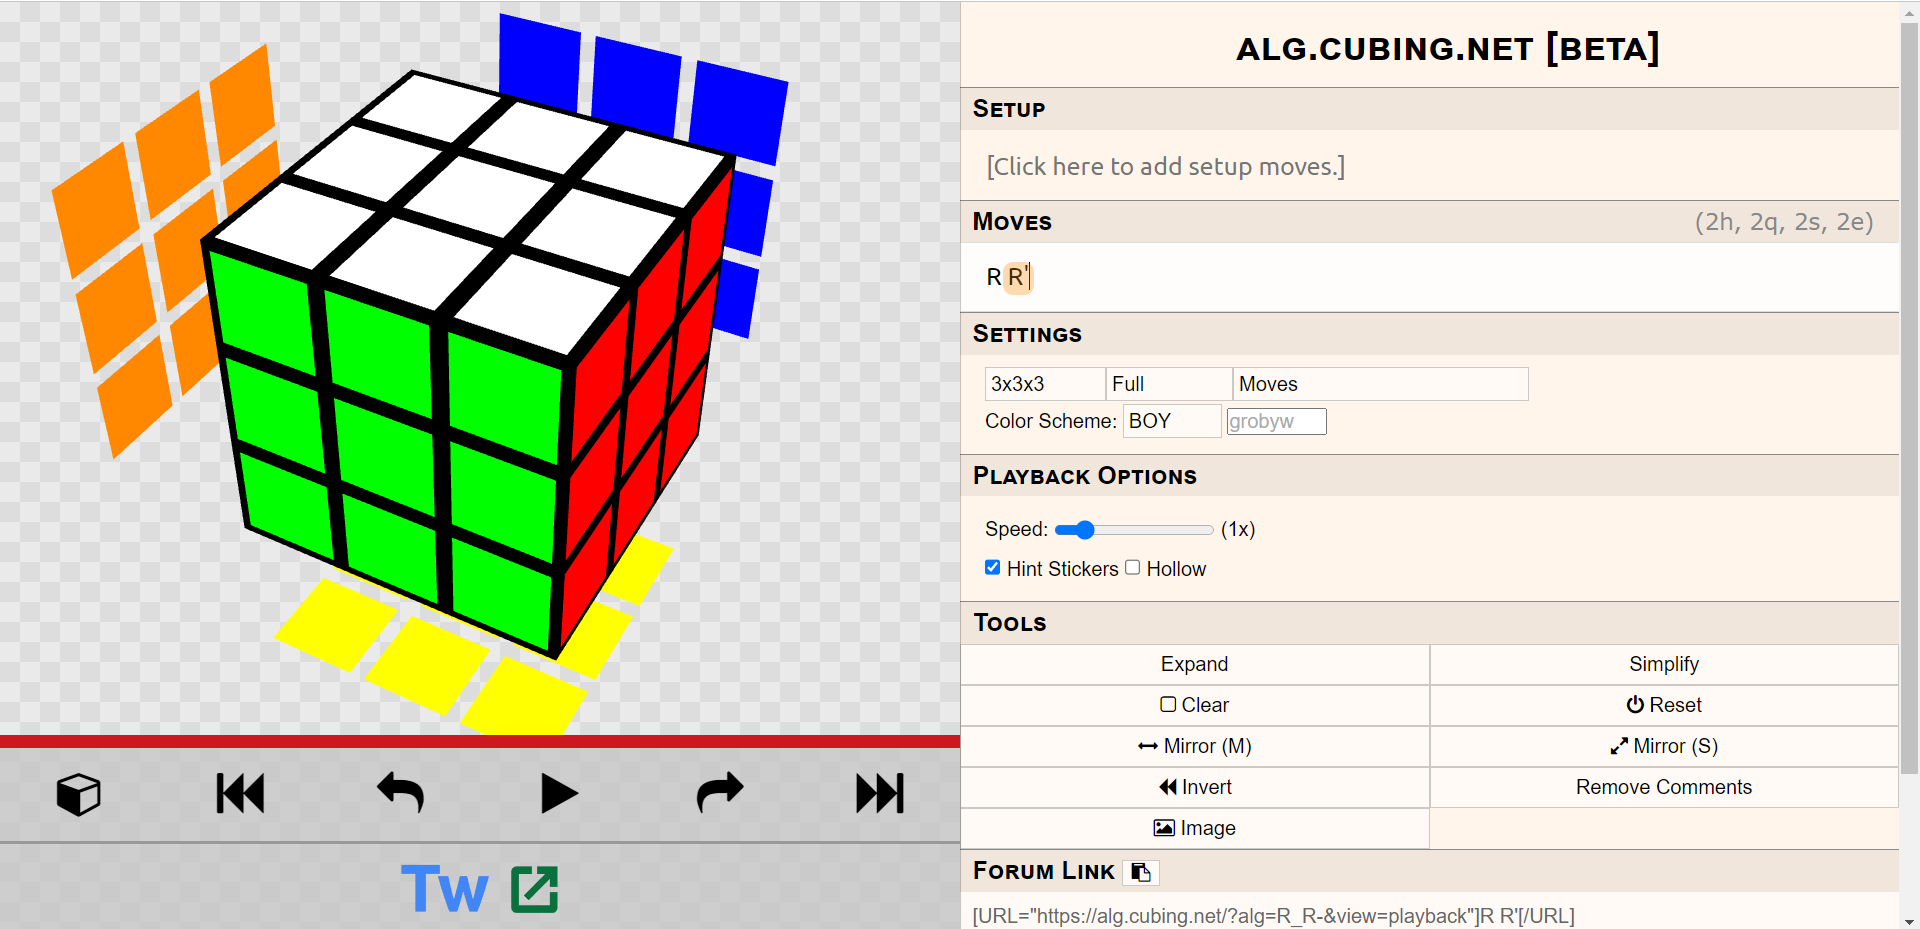
\includegraphics[width = 10cm ]{Screenshot 2023-07-06 005358.png}
    \caption{Performing its Inverse R'}
    \label{(RU R'U') R U or $ (a * b)*c $}
\end{figure}
Any move from $< R , L , U , D , F , B  >$ there exist an inverse element like as for $R$ its $R'$


.\\\\\\







\section{Permutations}
The puzzle was originally advertised as having "over 3,000,000,000 (three billion) combinations but only one solution". Depending on how combinations are counted, the actual number is significantly higher.
The original$ (3*3*3)$ Rubik's Cube has eight corners and twelve edges. There are $8!$ $(40,320)$ ways to arrange the corner cubes. Each corner has three possible orientations, although only seven (of eight) can be oriented independently; the orientation of the eighth (final) corner depends on the preceding seven, giving $3^{7} (2,187)$ possibilities. There are $12!/2 (239,500,800)$ ways to arrange the edges, restricted from 12! because edges must be in an even permutation exactly when the corners are. (When arrangements of centres are also permitted, as described below, the rule is that the combined arrangement of corners, edges, and centres must be an even permutation.) Eleven edges can be flipped independently, with the flip of the twelfth depending on the preceding ones, giving $2^{11} (2,048)$ possibilities.\cite{wong2010group}\\

\begin{center}
    $ 8! * 3^{7} * \frac{12!}{2} * 2^{11} $ = $43,252,003,274,489,856,0000$
\end{center}
which is approximately $43$ quintillion.\\
To put this into perspective, if the earth has a only one rubik's cube solver, if he or she averages $30$ seconds to solve and $15$ seconds to scramble and 15 seconds to solve 1 minute per permutation and he or she practices $24/7$ and no breaks at all ever that means she can solve $1440$ solve per day as$ 24 * 60 $min = $1440$ min. That's a lot for a average cuber. then the total number of scramble is $43,252,003,274,489,856,0000$ then the number of days he or she need is\\
\begin{center}
   $\frac{43252003274489856000}{1440}=300361133850624000$.  number of days.\\
\end{center}

if we divide this with $365$ days then the number of year we got $822907216029106.849315$ or $8.229072 * 10^{14}$ which is \textbf{Eight hundred twenty-two trillion nine hundred seven billion two hundred sixteen million twenty-nine thousand one hundred nine and nine trillion eight hundred ninety-one billion eighty-two million nine hundred twenty-two thousand one hundred thirteen ten-trillionths years}.\\
Basically it is impossible for one of us to solve all the scramble.\\
The Fun part is , the preceding figure is limited to permutations that can be reached solely by turning the sides of the cube. If one considers permutations reached through disassembly of the cube, the number becomes twelve times larger:
\begin{center}
     $ 8! * 3^{8} * {12!} * 2^{12} $ = $519,024,039,293,878,272,000$
\end{center}
which is approximately 519 quintillion[5] possible arrangements of the pieces that make up the cube, but only one in twelve of these are actually solvable. This is because there is no sequence of moves that will swap a single pair of pieces or rotate a single corner or edge cube. Thus, there are 12 possible sets of reachable configurations, sometimes called "universes" or "orbits", into which the cube can be placed by dismantling and reassembling it.

The preceding numbers assume the centre faces are in a fixed position. If one considers turning the whole cube to be a different permutation, then each of the preceding numbers should be multiplied by 24. A chosen colour can be on one of six sides, and then one of the adjacent colours can be in one of four positions; this determines the positions of all remaining colours.
\section{Solution to The Rubik's Cube}
The most used algorithm is Beginner's Method.which is basically layer by layer method.\\
There many speed cubers around the world and the most common is the CFOP ,Petrus ,Roux , ZZ Method.But the most popular is CFOP, Which is developed by  Jessica Fridrich. This method is called CFOP standing for "cross, F2L, OLL, PLL". It is similar to the layer-by-layer method but employs the use of a large number of algorithms, especially for orienting and permuting the last layer. The cross is done first, followed by first layer corners and second layer edges simultaneously, with each corner paired up with a second-layer edge piece, thus completing the first two layers (F2L). This is then followed by orienting the last layer, then permuting the last layer (OLL and PLL respectively). Fridrich's solution requires learning roughly 120 algorithms but allows the Cube to be solved in only 55 moves on average.\\
\subsection{Optimal solutions for Rubik's Cube}
Optimal solutions for Rubik's Cube refer to solutions that are the shortest. There are two common ways to measure the length of a solution. The first is to count the number of quarter turns. The second is to count the number of outer-layer twists, called "face turns". A move to turn an outer layer two quarter (90°) turns in the same direction would be counted as two moves in the quarter turn metric (QTM), but as one turn in the face metric (FTM, or HTM "Half Turn Metric", or OBTM "Outer Block Turn Metric").\cite{rokicki2010god}

The maximal number of face turns needed to solve any instance of the Rubik's Cube is 20,\cite{rokicki2010god} and the maximal number of quarter turns is 26.\cite{rokicki2010god} These numbers are also the diameters of the corresponding Cayley graphs of the Rubik's Cube group. In STM (slice turn metric), the minimal number of turns is unknown.

There are many algorithms to solve scrambled Rubik's Cubes. An algorithm that solves a cube in the minimum number of moves is known as God's algorithm.
\begin{itemize}
    \item Thistlethwaite's algorithm
    \item Kociemba's algorithm
    \item Korf's algorithm
    \item God's Number
\end{itemize}

\section{Conclusion}
In this paper, we attempted to demonstrate the algebraic combinatorics of the Rubik's cube.We have tried to find the relation between rubik's cube and mathematics more precisely with Group theory.The Rubik's cube contains many mysteries.We only find the god's number for 2*2*2 and 3*3*3 but not for large cubes.Hopefully, one day we will discover.







\bibliographystyle{plain}
\bibliography{references.bib}
\end{document}
